\chapter{Methodology}
\label{chap:met}

This chapter will present a detailed explanation of the principles underlying the 
proposed methodology. The section \ref{sec:rigid_body_and_const} offers a concise 
overview of rigid-body systems and constraints that can be imposed on them.
The next section \ref{sec:udwadia_kalaba_app} introduces the Udwadia-Kalaba 
approach and physical principles that stays behind it.

\section{Rigid-body systems and constraints} 
\label{sec:rigid_body_and_const}

The most common class of physical systems that can be observed in the real life 
cases is the rigid-body one. Some examples of such systems are demonstrated in 
Figure \ref{fig:examples_of_rig_sys}. The key feature of rigid-body systems 
is non-deformable parts that forms it. With these limitations only an 
inner stiffness can be described.

\begin{figure}[H]
    \centering
    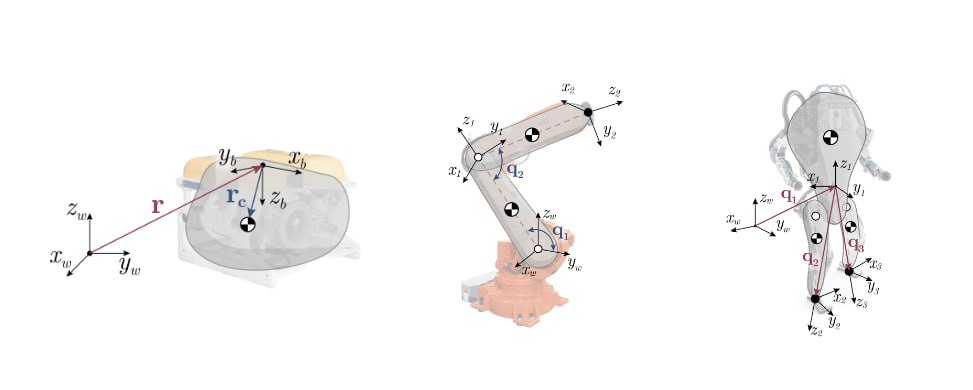
\includegraphics[scale=0.5]{figs/rigid_body_systems.png}
    \caption{Examples of rigid-body systems}
    \label{fig:examples_of_rig_sys}
\end{figure}


Nevertheless, the mathematical tools to work with rigid-body systems was introduced 
in \RNum{18}-th century by Newton and Euler works. Using this approach it is easy 
to formulate a set f deferential equations that describes the system behavior.
However, in this study the another (more convenient) technique is utilized. It is 
called the least action principle. The formulation is the following equation

\begin{equation}
    \min_{\mathbf{q}} \quad 
    \int_{t_1}^{t_2} L(\mathbf{q}(t), \mathbf{v}(t), t) dt
    \label{eqn:least_act_principle}
\end{equation}

where $L$ is Lagrangian of the system, and $\mathbf{q}$, $\mathbf{v}$ are 
functions of the generalized coordinates and velocities respectively. The solution 
of the variational problem (\ref{eqn:least_act_principle}) is the Euler-Lagrange 
differential equations. The solution through utilizing the Lagrangian can be 
easily generalized to all rigid-body systems. This generalization is aforementioned 
the canonical manipulator equation (\ref{eqn:can_man_equation}). 

In this chapter the convenient representation of this equation is used. The main 
idea of rewriting is combination of the inertial forces with non-inertial ones.

\begin{equation}
    M \dot{\mathbf{v}} = \mathbf{Q}
    \label{eqn:can_man_eqn_simple}
\end{equation}

In the above equation $\mathbf{Q} = 
-C(\mathbf{q}, \mathbf{v}) \dot{\mathbf{q}} - g(\mathbf{q}) + 
\boldsymbol{\tau}$, $M \succcurlyeq 0$ is inertia matrix, $C$ is Centrifugal-Coriolis 
matrix, $g$ is gradient of conservative forces. The dependency from coordinates and 
velocities is amended for convenience. In the most generalized case 
$\dim{\mathbf{q}} = n_q \neq n_v = \dim{\mathbf{v}}$.

The aforementioned description is applicable for open and closed loop systems. 
The closed one is described in Figure \ref{fig:rigid_coupling}. However, 
as mentioned above utilizing only equation \ref{eqn:can_man_eqn_simple} to handle 
such system is not efficient. Thus, the approach via constraints described
by equation (\ref{eqn:holonom_const}) is more preferable. It can be inserted in 
(\ref{eqn:least_act_principle}), which leads to the following variational problem, 

\begin{equation}
    \min_{\mathbf{q}} \quad 
    \int_{t_1}^{t_2} [L(\mathbf{q}(t), \mathbf{v}(t), t) - 
    \pmb{\lambda}^T \varphi(\mathbf{q}(t), t)]dt
    \label{eqn:least_act_principle_const}
\end{equation}

The solution the above equation can be expressed in terms of the KKT matrix in 
the following way, 

\begin{equation}
    \begin{bmatrix}
        M & J^T \\
        J & 0 \\
    \end{bmatrix}
    \begin{bmatrix}
        \dot{\mathbf{v}} \\
        -\pmb{\lambda}
    \end{bmatrix} = 
    \begin{bmatrix}
        \mathbf{Q} \\
        -\dot{J} \mathbf{v}
    \end{bmatrix}, \:
    J = \frac{\partial \boldsymbol{\varphi}}{\partial \mathbf{q}}
    \label{eqn:kkt_solution}
\end{equation}

The downside of the equation (\ref{eqn:kkt_solution}) is that it does not support 
non-holonomic constraints generally. This type of constraints can be defined as 

\begin{equation}
    \varphi(\mathbf{q}, \mathbf{v}, t) = 0
    \label{eqn:non_holonomic_const}
\end{equation}

Therefore, the dependency from generalized velocity makes the KKT approach not 
applicable. The handle of such constraints is crucial for defining a control. 
Hence, it is necessary to use another technique.

\section{The Udwadia-Kalaba approach} \label{sec:udwadia_kalaba_app}

The main differences of the Udwadia-Kalaba approach from the method mentioned 
above are the another view on constraints, and utilizing different physical 
principle.

Let's start from reviewing the constraints form in the discussed technique. It 
can be derived from holonomic and non-holonomic type by differentiating over time, 
and transforming to an affine form. The general equation is the following 

\begin{equation}
    A(\mathbf{q}, \mathbf{v}, t) \dot{\mathbf{v}} = 
    \mathbf{b}(\mathbf{q}, \mathbf{v}, t)
    \label{eqn:affine_const}
\end{equation}

The above equation can be used in the Gauss least constraint principle. For further 
convenience the arguments of matrix functions is amended. It leads to the 
following optimization problem:

\begin{equation}
    \begin{aligned}
        \min_{\dot{\mathbf{v}}} \quad &
        [\dot{\mathbf{v}} - \mathbf{a}]^T M [\dot{\mathbf{v}} - \mathbf{a}] \\
        \textrm{s.t.} \quad &
        A \dot{\mathbf{v}} = \mathbf{b} \\
        &
        \mathbf{a} = M^{-1} \mathbf{Q}
    \end{aligned}
    \label{eqn:gauss_least_const}
\end{equation}

This optimization can be solved analytically as Ferdaus Udwadia and Robert Kalaba 
demonstrated \cite{UdwadiaKalabaApproach}. This solution is shown below.

\begin{equation}
    \dot{\mathbf{v}} = 
    \mathbf{a} + M^{-1 / 2}(A M^{-1 / 2})^+ (\mathbf{b} - AM^{-1} \mathbf{Q})
    \label{eqn:udwadia_kalaba_sol}
\end{equation}

where $[\cdot]^+$ is the Moore-Penrose inverse, and 
$M^{\pm 1 / 2} = W \Lambda^{\pm 1 / 2} W^T$, $W$ is the orthogonal matrix 
of eigen vectors. 

In case of positive semi-definiteness of $M$ the equation 
(\ref{eqn:udwadia_kalaba_sol}) is not applicable because $M^{-1}$, 
$M^{-1 / 2}$ cannot exist. The Firdaus Udwadia and Aaron Schutte demonstrates 
\cite{EquationsOfMotionConst} a methodology to bypass this problem by 
replacing $M$, and $\mathbf{a}$ by the following quantities respectively

\begin{equation}
    \begin{aligned}
        M_A = M + A^+ A \succ 0 \\
        \mathbf{a}_A = M_A^{-1} \mathbf{Q}
    \end{aligned}
    \label{eqn:another_mass_matrix}
\end{equation}

Utilizing the mentioned quantities it is possible to define constraints 
force over the wide range of rigid-body systems. These forces can be 
expressed in the following manner 

\begin{equation}
    \mathbf{Q}_C = M^{1 / 2} (A M^{-1 /2})^+(\mathbf{b} - AM^{-1} \mathbf{Q})
    \label{eqn:constraint_forces}
\end{equation}

Hence, the Udwadia-Kalaba approach is applicable for emulation a of 
rigid body constraint in computation easily. Only the problem with rigorous 
defining $A$ and $\mathbf{b}$ remains.

\section{Defying constraints over multiple systems}

This section introduces a common holonomic constraint, which serves as a foundation 
for further investigations. This constraint delineates a rigid body's behavior, 
applicable to multiple manipulators.

Let $M_1, M_2, \dots, M_p$ are $p$ iinertia matrices for $p$ independent systems. 
The $i$-th system has $n_q^i$ generalized coordinates, $n_v^i$ generalized velocity 
components and $Q_i$ bias force. Thus, the common unconstrained dynamics is

\begin{equation}
    \label{eqn:common_dynamics}
    \begin{bmatrix}
        M_1 & 0   & \dots & 0 \\
        0   & M_2 & \dots & 0 \\
        \vdots & \vdots & \ddots & \vdots \\
        0   & 0   & \dots & M_p
    \end{bmatrix}
    \begin{bmatrix}
        \ddot{\mathbf{q}}_1 \\ \ddot{\mathbf{q}}_2 \\ \vdots \\ \ddot{\mathbf{q}}_p
    \end{bmatrix}
    = 
    \begin{bmatrix}
        Q_1 \\ Q_2 \\ \vdots \\ Q_p
    \end{bmatrix}
\end{equation}

The equation \ref{eqn:common_dynamics} can be rewriten in the manner of
\ref{eqn:compact_man_eq}. In such compact form it is convinient for futher analysis. 
Hense, let

\begin{equation}
    \label{eqn:common_mass}
    M_s = 
    \begin{bmatrix}
        M_1 & 0   & \dots & 0 \\
        0   & M_2 & \dots & 0 \\
        \vdots & \vdots & \ddots & \vdots \\
        0   & 0   & \dots & M_p
    \end{bmatrix}
\end{equation}

\begin{equation}
    \label{eqn:common_q}
    q_s = 
    \begin{bmatrix}
        \mathbf{q}_1 & \mathbf{q}_2 & \dots & \mathbf{q}_p
    \end{bmatrix}^T
\end{equation}

\begin{equation}
    \label{eqn:common_bias}
    Q_s = 
    \begin{bmatrix}
        Q_1 & Q_2 & \dots & Q_p
    \end{bmatrix}^T
\end{equation}

It implies to the following dynamics equation that describes motion of $p$ independent 
systems

\begin{equation}
    \label{eqn:common_eq}
    M_s \ddot{\mathbf{q}}_s = \mathbf{Q}_s
\end{equation}

Let $R_{ij}$ and $\mathbf{p}_{ij}$ are rotation and position of $j$-th frame attached to some 
link of the $i$-th system respectevly. The rigid body connection between two frames 
now can be defined as

\begin{numcases}{}
    R_{ij}R_d = R_{\alpha \beta} & \label{eqn:rot_const}
    \\
    (\mathbf{p}_{ij} - \mathbf{p}_{\alpha \beta})^T
    (\mathbf{p}_{ij} - \mathbf{p}_{\alpha \beta}) = l & \label{eqn:position_const}
\end{numcases}

where $R_d$ is a fixed rotation matrix and $l$ a distence between connection points 
inside a rigid body.

Substituting 
$\prescript{\alpha \beta}{ij}{\mathbf{d}} = \mathbf{p}_{ij} - \mathbf{p}_{\alpha \beta}$ 
and differencing respect to time twice the equation \ref{eqn:position_const}
transforms to 

\begin{equation}
    \label{eqn:pos_const_transform_1}
    \prescript{\alpha \beta}{ij}{\mathbf{d}}^T 
    \prescript{\alpha \beta}{ij}{\mathbf{d}} - l = 0
    \Rightarrow
    \prescript{\alpha \beta}{ij}{\mathbf{d}}^T 
    \prescript{\alpha \beta}{ij}{\dot{\mathbf{d}}} = 0
    \Rightarrow
    \prescript{\alpha \beta}{ij}{\mathbf{d}}^T 
    \prescript{\alpha \beta}{ij}{\ddot{\mathbf{d}}} + 
    \prescript{\alpha \beta}{ij}{\dot{\mathbf{d}}}^T 
    \prescript{\alpha \beta}{ij}{\dot{\mathbf{d}}} = 0
\end{equation}

The equation \ref{eqn:pos_const_transform_1} can be expresed via generalized coordinates

\begin{equation}
    \label{eqn:pos_const_transform_2}
    \prescript{\alpha \beta}{ij}{\mathbf{d}}^T 
    \prescript{\alpha \beta}{ij}{\ddot{\mathbf{d}}} + 
    \prescript{\alpha \beta}{ij}{\dot{\mathbf{d}}}^T 
    \prescript{\alpha \beta}{ij}{\dot{\mathbf{d}}} = 0
    \Rightarrow
    \prescript{\alpha \beta}{ij}{\mathbf{d}}^T 
    (
        \prescript{v}{ij}{J} \ddot{\mathbf{q}}_s + 
        \prescript{v}{ij}{\dot{J}} \dot{\mathbf{q}}_s
    ) + 
    \dot{\mathbf{q}}_s^T \prescript{v}{ij}{J}^T 
    \prescript{v}{ij}{J} \dot{\mathbf{q}}_s = 0
\end{equation}

where $\prescript{v}{ij}{J} \equiv \prescript{v}{ij}{J}(\mathbf{q}_s)$ is the 
$j$-th frame velocity Jacobian of the $i$-th system. Now, it is possible to 
convert \ref{eqn:position_const} constraint to \ref{eqn:udwadia_const_form} form

\begin{equation}
    \label{eqn:pos_const_a_matrix}
    A_p(\mathbf{q}_s, \dot{\mathbf{q}}_s) = 
    \prescript{\alpha \beta}{ij}{\mathbf{d}}^T \prescript{v}{ij}{J}
\end{equation}

\begin{equation}
    \label{eqn:pos_const_b_vector}
    b_p(\mathbf{q}_s, \dot{\mathbf{q}}_s) = 
    - \prescript{\alpha \beta}{ij}{\mathbf{d}}^T 
    \prescript{v}{ij}{\dot{J}} \dot{\mathbf{q}}_s
    - \dot{\mathbf{q}}_s^T \prescript{v}{ij}{J}^T
    \prescript{v}{ij}{J} \dot{\mathbf{q}}_s
\end{equation}

Now, let suppose that $\gamma_1, \gamma_2, \dots, \gamma_w$ system connected by rigid 
body. Here $\gamma_i$ is an index of the system, and $w \leq p$. 
